\section{Lưu ý}
\begin{itemize}
\item Tài liệu này \textbf{không phải} là tài liệu chính thức của trường THPT Chuyên Bảo Lộc hay Đại học Quốc gia Thành phố Hồ Chí Minh.
\item Các hình ảnh, bảng biểu, hướng dẫn trong tài liệu \textbf{chỉ mang tính chất ví dụ}.
\item Các tài liệu kèm theo \textbf{không phải} của tác giả. Tác giả \textbf{không chịu trách nhiệm} với bất kì sai sót nào trong các tài liệu kèm theo.
\item Tác giả phân phối \textbf{miễn phí} tài liệu này \href{https://github.com/ductai05/DGNL_2024}{trên GitHub} với \href{https://github.com/ductai05/DGNL_2024/blob/main/LICENSE}{Giấy phép GNU General Public License v3.0}. 
\item Tài liệu được viết từ ngày 27/11/2023 đến ngày 29/01/2024.
\item Mọi \textbf{góp ý} xin hãy liên hệ trực tiếp đến tác giả: \href{https://facebook.com/ductai05}{Đinh Đức Tài}
\end{itemize}
\section{Hình ảnh}
\begin{figure}
    \centering
    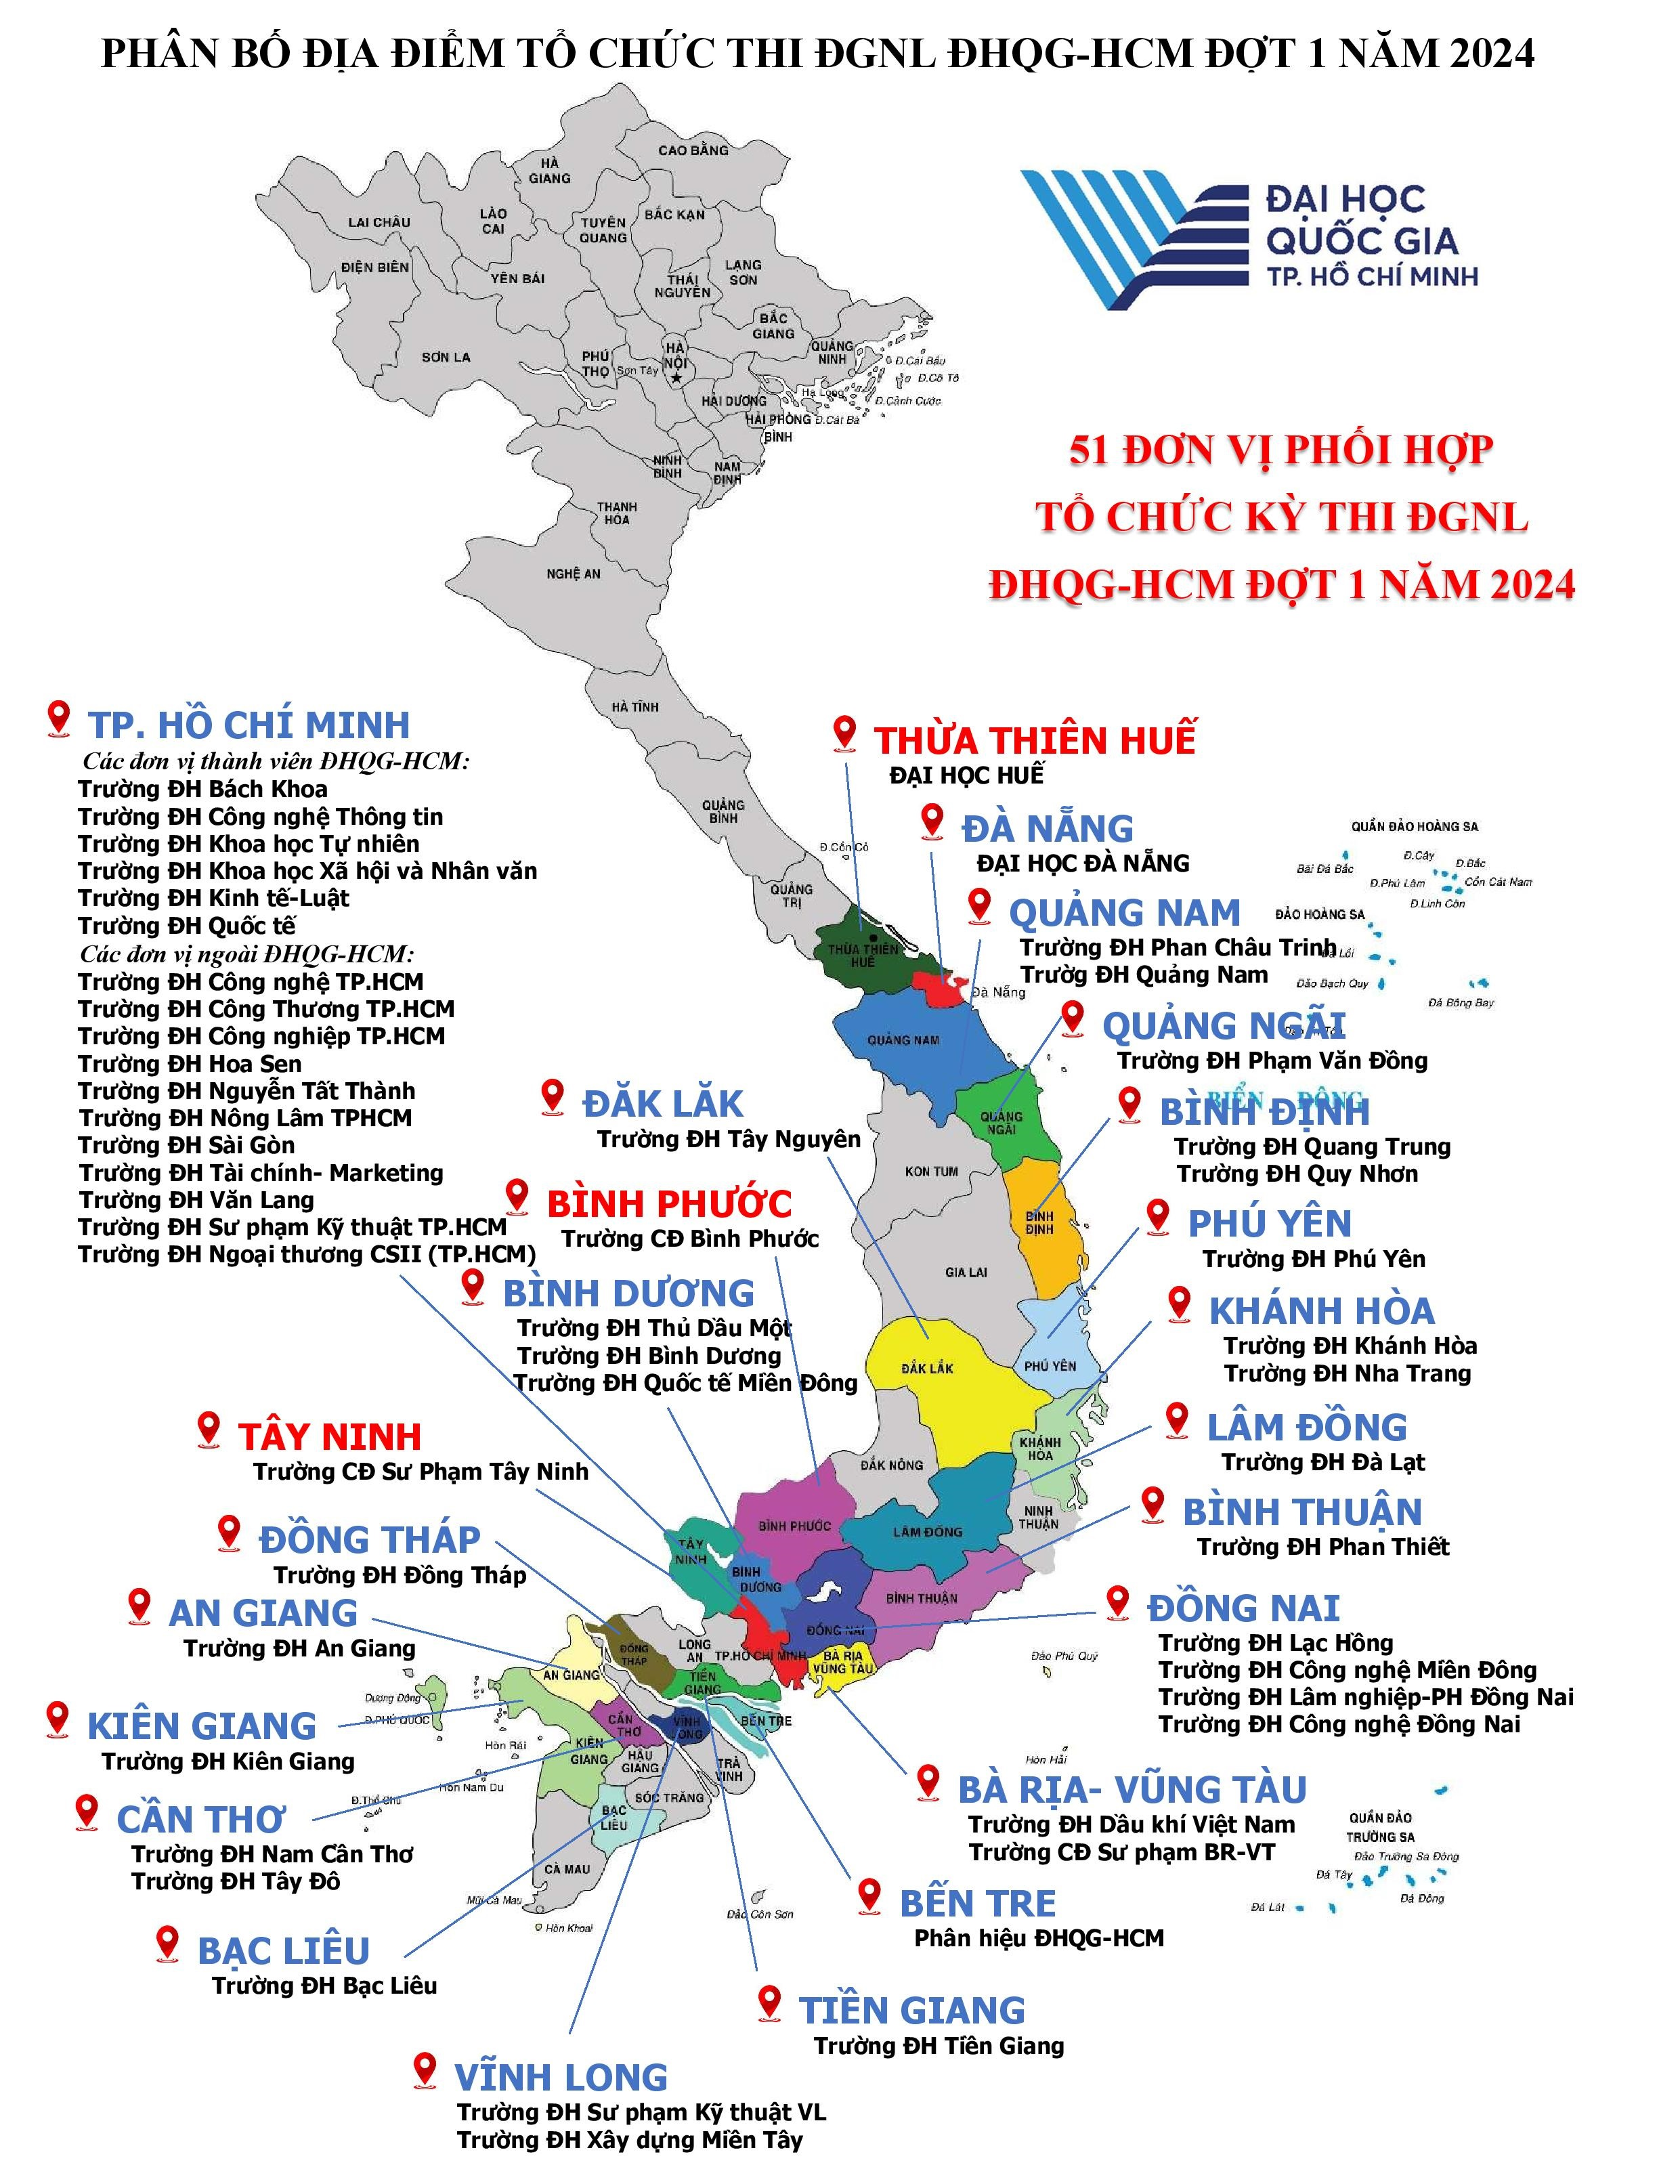
\includegraphics[width=1\linewidth]{img/Phan-bo-diem-thi-DGNL-Dot-1-2024.jpg}
    \caption{Phân bố điểm thi ĐGNL Đợt 1 - 2024}
    \label{fig:phanbodiemthi_dot1}
\end{figure}
\newpage
\section{Về tác giả}
\textbf{Thông tin cá nhân:}
\begin{itemize}
    \item Họ tên: Đinh Đức Tài
    \item Cựu học sinh chuyên Toán, TK9-CBL
    \item Sinh viên lớp AI-K2023, FIT@HCMUS, ĐHQG TP.HCM
    \item Top 0,244\% APT 2023 (1012đ); Top 2 HSG tỉnh Lâm Đồng - Toán 12, 2022 - 2023.
\end{itemize}
\textbf{Thông tin liên hệ:}
\begin{itemize}
    \item Facebook: \href{fb.com/ductai05}{fb.com/ductai05}
    \item GitHub: \href{github.com/ductai05}{github.com/ductai05}
\end{itemize}
\textbf{Repo GitHub - mã nguồn LaTeX của tài liệu:} 
\begin{itemize}
    \item \href{github.com/ductai05/StudyGuide_APT2024}{github.com/ductai05/StudyGuide\_APT2024}
\end{itemize}
\textbf{Phiên bản tài liệu: 1.0}
\begin{itemize}
    \item Ngày cập nhật: 28/01/2024
    \item Phiên bản mới nhất của tài liệu sẽ được cập nhật trên Repo GitHub.
\end{itemize}
